% ============================================================================
% LiteForge -- VDI / WSL Install and Quickstart Guide
% LiteForge
% ============================================================================
\documentclass[11pt,letterpaper]{article}

% --- Packages ---
\usepackage[T1]{fontenc}
\usepackage[utf8]{inputenc}
\usepackage[margin=1in]{geometry}
\usepackage{fancyhdr}
\usepackage[dvipsnames,table]{xcolor}
\usepackage{booktabs}
\usepackage{listings}
\usepackage[colorlinks=true]{hyperref}
\usepackage{tikz}
\usepackage[most]{tcolorbox}
\usepackage{tabularx}
\usepackage{enumitem}
\usepackage{parskip}
\usepackage{lmodern}
\usepackage{helvet}
\renewcommand{\familydefault}{\sfdefault}
\usepackage{graphicx}
\usepackage{titlesec}
\usepackage{setspace}
\usepackage{float}
\usepackage[font=small,labelfont=bf]{caption}

\usetikzlibrary{
  arrows.meta,positioning,shapes.geometric,fit,backgrounds,calc,
  decorations.pathreplacing,shapes.multipart,chains,matrix
}

% ---- Walter palette (light background) ----
\definecolor{navybg}{HTML}{0E2841}
\definecolor{navylight}{HTML}{152F4A}
\definecolor{walterpurple}{HTML}{715ABF}
\definecolor{walterorange}{HTML}{F08940}
\definecolor{walterdarkpurple}{HTML}{503F86}
\definecolor{copper}{HTML}{B86B4A}
\definecolor{recgreen}{HTML}{5AAF42}
\definecolor{alertred}{HTML}{B71C1C}
\definecolor{tipblue}{HTML}{2A7AB5}
\definecolor{tipgreen}{HTML}{5AAF42}
\definecolor{tiporange}{HTML}{F08940}
\definecolor{tipred}{HTML}{DC2626}
\definecolor{forgegray}{HTML}{666666}
\definecolor{lightgray}{HTML}{F5F5F5}
\definecolor{bordergray}{HTML}{DDDDDD}
\definecolor{codebg}{HTML}{F5F5F5}
\definecolor{codeframe}{HTML}{DDDDDD}

% --- Light page (white bg, navy text) ---
\color{navybg}
\arrayrulecolor{bordergray}
\hypersetup{linkcolor=tipblue, urlcolor=tipblue, citecolor=tipblue}

% --- Section heading colors ---
\titleformat{\section}
  {\Large\bfseries\color{navybg}}{\thesection}{1em}{}
\titleformat{\subsection}
  {\large\bfseries\color{walterpurple}}{\thesubsection}{1em}{}
\titleformat{\subsubsection}
  {\normalsize\bfseries\color{tipblue}}{\thesubsubsection}{1em}{}

% --- tcolorbox styles ---
\tcbset{
  tipbox/.style={
    enhanced, colback=tipgreen!5, colframe=tipgreen!50,
    colbacktitle=tipgreen!80, coltitle=white, coltext=navybg,
    fonttitle=\bfseries, title=#1,
    boxrule=0.5pt, arc=2pt, toptitle=4pt, bottomtitle=4pt,
    left=8pt, right=8pt, top=6pt, bottom=6pt,
  },
  warnbox/.style={
    enhanced, colback=alertred!5, colframe=alertred!50,
    colbacktitle=alertred!80, coltitle=white, coltext=navybg,
    fonttitle=\bfseries, title=#1,
    boxrule=0.5pt, arc=2pt, toptitle=4pt, bottomtitle=4pt,
    left=8pt, right=8pt, top=6pt, bottom=6pt,
  },
  infobox/.style={
    enhanced, colback=tipblue!5, colframe=tipblue!50,
    colbacktitle=tipblue!80, coltitle=white, coltext=navybg,
    fonttitle=\bfseries, title=#1,
    boxrule=0.5pt, arc=2pt, toptitle=4pt, bottomtitle=4pt,
    left=8pt, right=8pt, top=6pt, bottom=6pt,
  },
  notebox/.style={
    enhanced, colback=walterpurple!5, colframe=walterpurple!40,
    colbacktitle=walterpurple!80, coltitle=white, coltext=navybg,
    fonttitle=\bfseries, title=#1,
    boxrule=0.5pt, arc=2pt, toptitle=4pt, bottomtitle=4pt,
    left=8pt, right=8pt, top=6pt, bottom=6pt,
  },
  stepbox/.style={
    enhanced, colback=walterorange!5, colframe=walterorange!50,
    colbacktitle=walterorange!80, coltitle=white, coltext=navybg,
    fonttitle=\bfseries, title=#1,
    boxrule=0.5pt, arc=2pt, toptitle=4pt, bottomtitle=4pt,
    left=8pt, right=8pt, top=6pt, bottom=6pt,
  },
}

% --- Listings ---
\lstset{
  basicstyle=\ttfamily\small\color{navybg},
  backgroundcolor=\color{codebg},
  frame=single,
  rulecolor=\color{codeframe},
  breaklines=true,
  breakatwhitespace=false,
  breakautoindent=true,
  columns=fullflexible,
  keepspaces=true,
  showstringspaces=false,
  tabsize=2,
  xleftmargin=4pt,
  xrightmargin=4pt,
  aboveskip=8pt,
  belowskip=8pt,
}

\lstdefinestyle{bash}{
  language=bash,
  keywordstyle=\color{tipblue}\bfseries,
  stringstyle=\color{tipgreen},
  commentstyle=\color{forgegray}\itshape,
  morekeywords={sudo,apt,git,curl,cargo,source,forge,claude,wsl},
}

\lstdefinestyle{powershell}{
  language={},
  keywordstyle=\color{tipblue}\bfseries,
  morekeywords={wsl,PS},
}

% --- Header / Footer ---
\pagestyle{fancy}
\fancyhf{}
\fancyhead[L]{\small\color{forgegray}LiteForge -- WSL / Linux / macOS Install Guide}
\fancyhead[R]{\small\color{forgegray}LiteForge}
\fancyfoot[C]{\small\color{forgegray}\thepage}
\fancyfoot[R]{\tiny\color{alertred}\textit{Proprietary and Confidential}}
\renewcommand{\headrulewidth}{0.4pt}
\renewcommand{\footrulewidth}{0.2pt}

% --- Graphics path ---
\graphicspath{{images/}}

% ============================================================================
\begin{document}

% ---- Title Page ----
\begin{titlepage}
\centering
\vspace*{2cm}

{\Huge\bfseries\color{navybg}LiteForge}\\[6pt]
{\Large\color{walterpurple}WSL / Linux / macOS Install and Quickstart Guide}

\vspace{1.5cm}


\begin{tikzpicture}
  \draw[walterorange, line width=2pt] (0,0) -- (10,0);
\end{tikzpicture}

\vspace{1.5cm}

{\large Sean Poyner}\\[4pt]
{\normalsize\color{forgegray}Senior Director, AI Engineering (Use Case)}\\[4pt]
{\normalsize\color{forgegray}Data, AI \& Emerging Technology Guild}\\[12pt]
{\normalsize LiteForge}

\vspace{1.5cm}

{\normalsize April 2026}

\vfill

{\small\color{alertred}\textbf{LiteForge}}
\end{titlepage}

% ---- Table of Contents ----
\tableofcontents
\newpage

% ============================================================================
\section{Overview}
% ============================================================================

The \textbf{Travel Innovation Platform (LiteForge) SDK} provides a CLI tool
(\texttt{forge}), Python, JavaScript, and Rust SDKs, and an Agent Development
Kit for building AI-powered applications on internal LLM
gateway.

This guide walks through installing the LiteForge on three Unix-style
environments:
\begin{itemize}[nosep]
  \item \textbf{WSL} (Windows Subsystem for Linux) on a VDI ---
    the recommended path on Windows
  \item \textbf{Linux} (Ubuntu / Debian) on bare metal or in a container
  \item \textbf{macOS} on Apple silicon or Intel hardware
\end{itemize}
By the end you will have a working \texttt{forge} CLI, the Python SDK, and
Claude Code integration that points at the LiteForge gateway.

\begin{tcolorbox}[infobox={Prerequisites}]
\textbf{Hardware / OS}
\begin{itemize}[nosep]
  \item One of: Windows 10/11 with WSL\,2, Ubuntu 22.04+ / Debian 12+, or
    macOS 13+ (Ventura or newer)
  \item x86\_64 or aarch64 (Apple silicon supported)
  \item $\sim$5\,GB free disk for Rust toolchain, build artifacts, and
    crate cache
  \item Internet access to \texttt{gitea.poyner.ai}, \texttt{crates.io},
    \texttt{pypi.org}, \texttt{nodejs.org}, and (for Mac) \texttt{brew.sh}
\end{itemize}
\textbf{Accounts \& credentials}
\begin{itemize}[nosep]
  \item GitHub Enterprise credentials (\texttt{gitea.poyner.ai})
  \item LiteForge API key (obtain from your team lead or the LiteForge.ai portal ---
    starts with \texttt{sk-z-})
\end{itemize}
\textbf{Tools the installer assumes are available} (Step~2 covers each)
\begin{itemize}[nosep]
  \item \texttt{git} --- to clone the repo
  \item \texttt{curl} --- to download \texttt{rustup}
  \item C toolchain (\texttt{cc} / \texttt{clang}) --- Rust links native
    code
  \item OpenSSL development headers --- some crate build scripts
  \item \texttt{python3} ($\geq$3.10) and \texttt{pip} --- for
    \texttt{liteforge-py}
  \item \texttt{node} and \texttt{npm} (LTS) --- \emph{optional}, for
    \texttt{liteforge-js}
  \item \texttt{cargo} (Rust 1.75+) --- installed in Step~3
\end{itemize}
\textbf{Administrator / sudo access}
\begin{itemize}[nosep]
  \item Windows: Administrator (one-time, for \texttt{wsl --install})
  \item Linux: \texttt{sudo} for \texttt{apt-get install}
  \item macOS: standard user is sufficient if Homebrew is already
    installed; otherwise admin password for the Homebrew install
\end{itemize}
\end{tcolorbox}

\newpage
% ============================================================================
\section{Step 1: Open a Shell}
% ============================================================================

\subsection{Windows: Enable WSL}

If you are on Windows and do not yet have WSL, open \textbf{PowerShell as
Administrator} and run:

\begin{lstlisting}[style=powershell]
wsl --install
\end{lstlisting}

\begin{figure}[H]
\centering
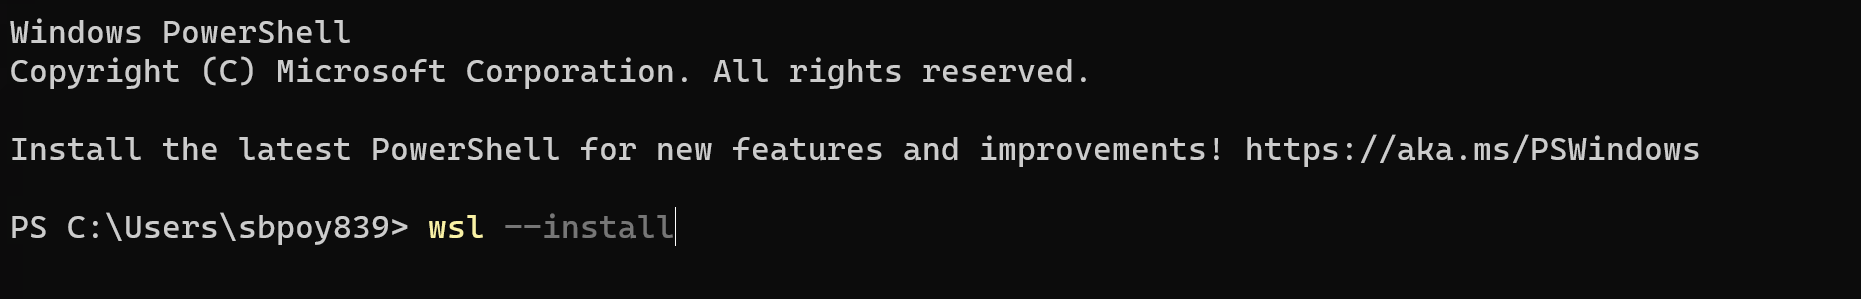
\includegraphics[width=0.85\textwidth]{slide01_img00.png}
\caption{Running \texttt{wsl --install} in PowerShell on the VDI.}
\end{figure}

This installs the WSL\,2 kernel and Ubuntu as the default distribution.
\textbf{Restart the VDI} when prompted. After reboot, Ubuntu will finish
its first-time setup and ask you to create a Unix username and password.
For the rest of this guide, all commands run inside the
\textbf{Ubuntu (WSL)} terminal.

\begin{tcolorbox}[notebox={Note}]
If WSL is already installed, skip this step. Verify with
\texttt{wsl --status} in PowerShell.
\end{tcolorbox}

\subsection{Linux: open your terminal}

No setup required --- open your normal terminal application
(\texttt{gnome-terminal}, \texttt{konsole}, \texttt{xterm}, etc.). Skip
straight to Step~2.

\subsection{macOS: open Terminal}

Open the \textbf{Terminal} app (or iTerm2). The macOS path uses
\textbf{Homebrew} for system dependencies. If Homebrew is not installed,
install it first:

\begin{lstlisting}[style=bash]
/bin/bash -c "$(curl -fsSL https://raw.githubusercontent.com/Homebrew/install/HEAD/install.sh)"
\end{lstlisting}

Then add it to your shell PATH (the installer prints the exact lines, but
typically):

\begin{lstlisting}[style=bash]
# Apple silicon (M1/M2/M3/M4)
echo 'eval "$(/opt/homebrew/bin/brew shellenv)"' >> ~/.zprofile
eval "$(/opt/homebrew/bin/brew shellenv)"
\end{lstlisting}

\begin{tcolorbox}[notebox={Apple silicon vs Intel}]
On Apple silicon, Homebrew lives at \texttt{/opt/homebrew}. On Intel
Macs, it lives at \texttt{/usr/local}. The \texttt{brew shellenv} command
prints the right \texttt{eval} line for your machine.
\end{tcolorbox}

\newpage
% ============================================================================
\section{Step 2: Install System Dependencies}
% ============================================================================

Install the packages required by the LiteForge build toolchain. Pick the
section that matches your environment.

\subsection{WSL / Ubuntu / Debian}

\begin{lstlisting}[style=bash]
sudo apt-get update
sudo apt-get install -y \
    build-essential \
    pkg-config \
    libssl-dev \
    python3-pip \
    python3-venv \
    curl \
    git
\end{lstlisting}

For the optional JavaScript SDK, also install Node.js LTS via NodeSource:

\begin{lstlisting}[style=bash]
curl -fsSL https://deb.nodesource.com/setup_20.x | sudo -E bash -
sudo apt-get install -y nodejs
\end{lstlisting}

\subsection{macOS (Homebrew)}

\begin{lstlisting}[style=bash]
brew install pkg-config openssl@3 python@3.12 git
\end{lstlisting}

A C toolchain is bundled with Xcode Command Line Tools. If
\texttt{cc --version} fails, install them:

\begin{lstlisting}[style=bash]
xcode-select --install
\end{lstlisting}

For the optional JavaScript SDK:

\begin{lstlisting}[style=bash]
brew install node
\end{lstlisting}

\begin{tcolorbox}[warnbox={Why these packages?}]
\begin{itemize}[nosep]
  \item \textbf{C toolchain} (\texttt{build-essential} on apt, Xcode CLT
    on macOS) --- provides \texttt{cc}/\texttt{clang}, required by Rust to
    link native code. Without it Rust fails with
    \texttt{error: linker `cc' not found}.
  \item \textbf{\texttt{pkg-config}, OpenSSL headers} --- needed by some
    Rust crate build scripts (\texttt{libssl-dev} on apt,
    \texttt{openssl@3} on Homebrew).
  \item \textbf{Python 3 + pip} --- required for the Python SDK install
    (\texttt{python3-pip}, \texttt{python3-venv} on apt;
    \texttt{python@3.12} on Homebrew). Without pip the install fails with
    \texttt{No module named pip}.
  \item \textbf{\texttt{curl}, \texttt{git}} --- for downloading Rust and
    cloning the repository.
  \item \textbf{Node.js LTS} (optional) --- needed only if you want
    \texttt{liteforge-js}.
\end{itemize}
\end{tcolorbox}

\newpage
% ============================================================================
\section{Step 3: Install Rust}
% ============================================================================

Install the Rust toolchain via \texttt{rustup}:

\begin{lstlisting}[style=bash]
curl --proto '=https' --tlsv1.2 -sSf https://sh.rustup.rs | sh
\end{lstlisting}

\begin{figure}[H]
\centering
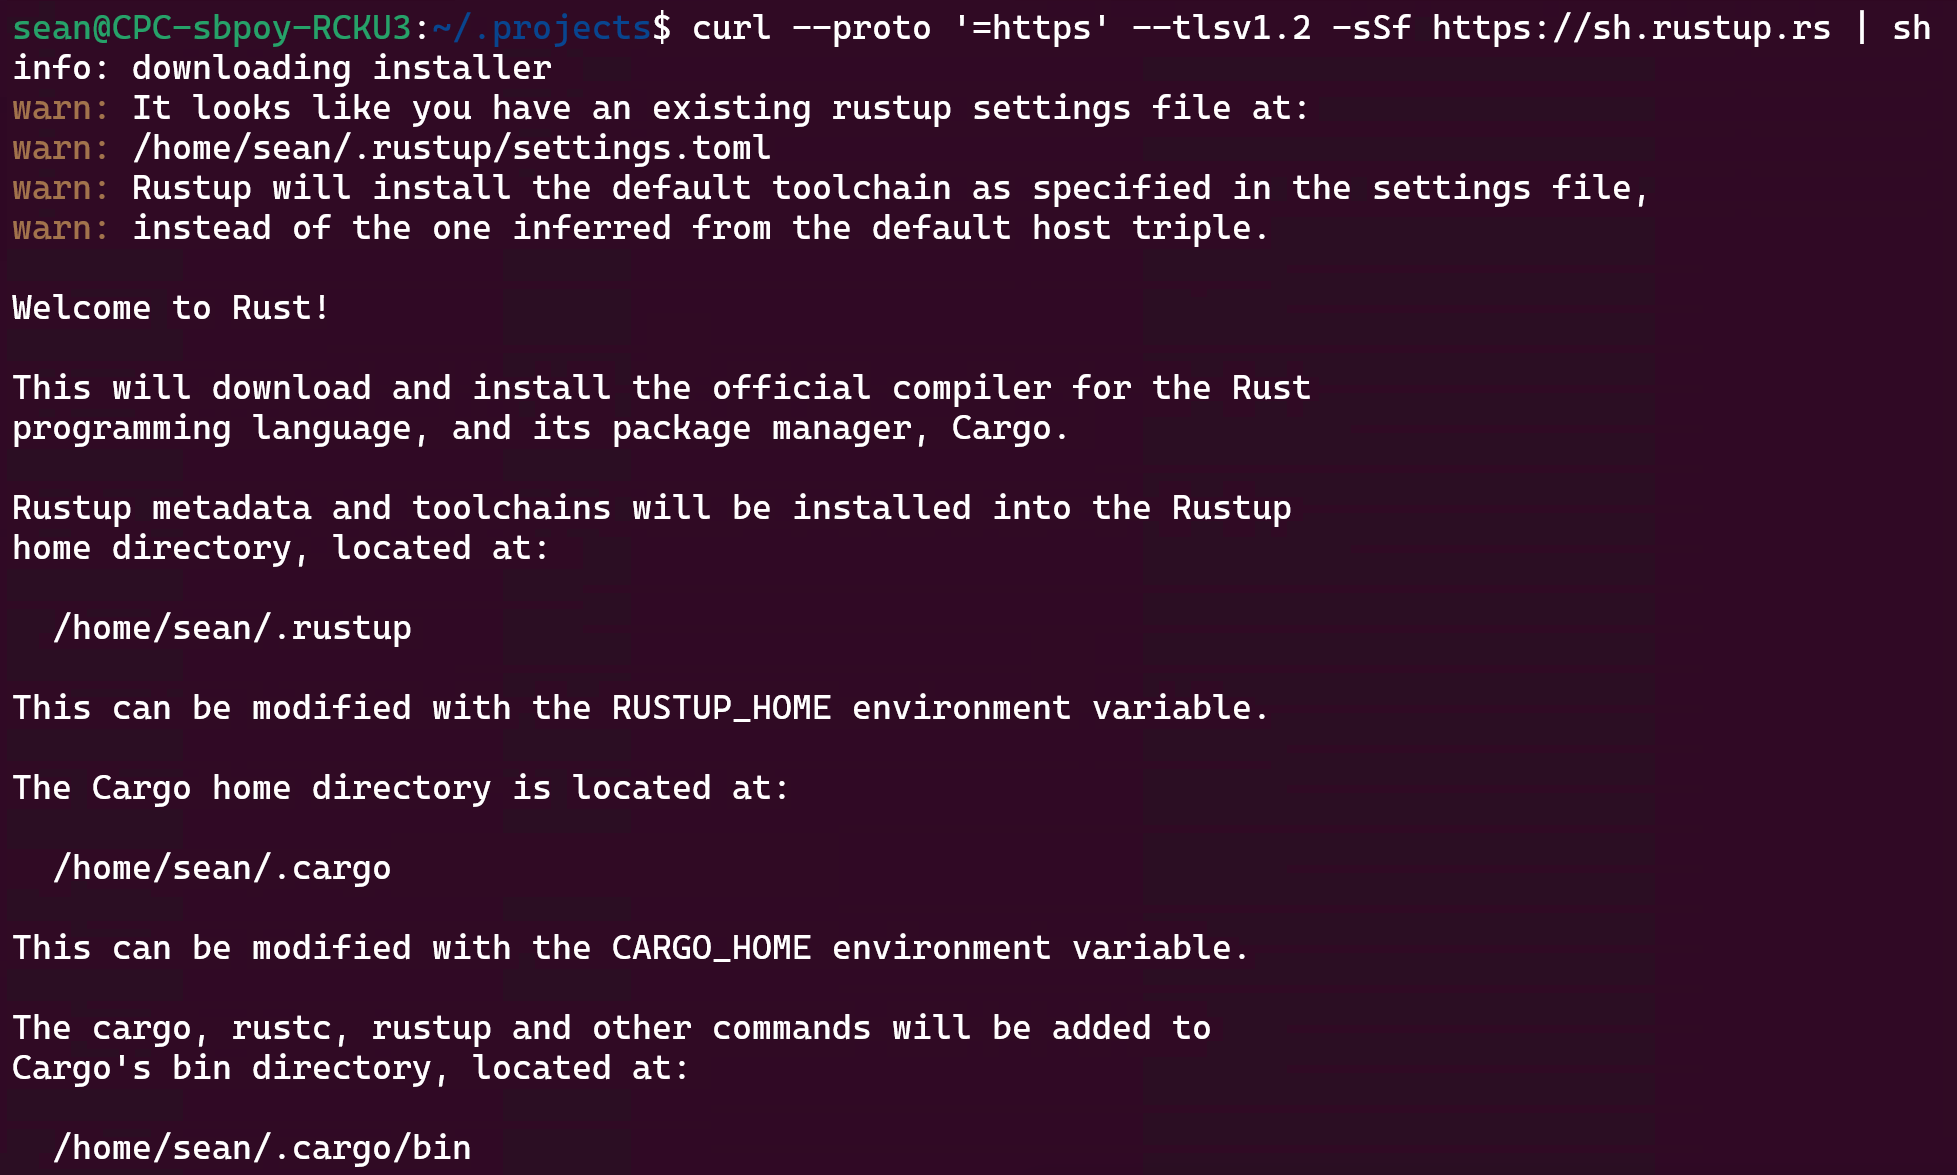
\includegraphics[width=0.85\textwidth]{slide02_img01.png}
\caption{The Rustup installer downloads and displays installation options.}
\end{figure}

When prompted, select \textbf{option 1} (``Proceed with standard
installation''):

\begin{figure}[H]
\centering
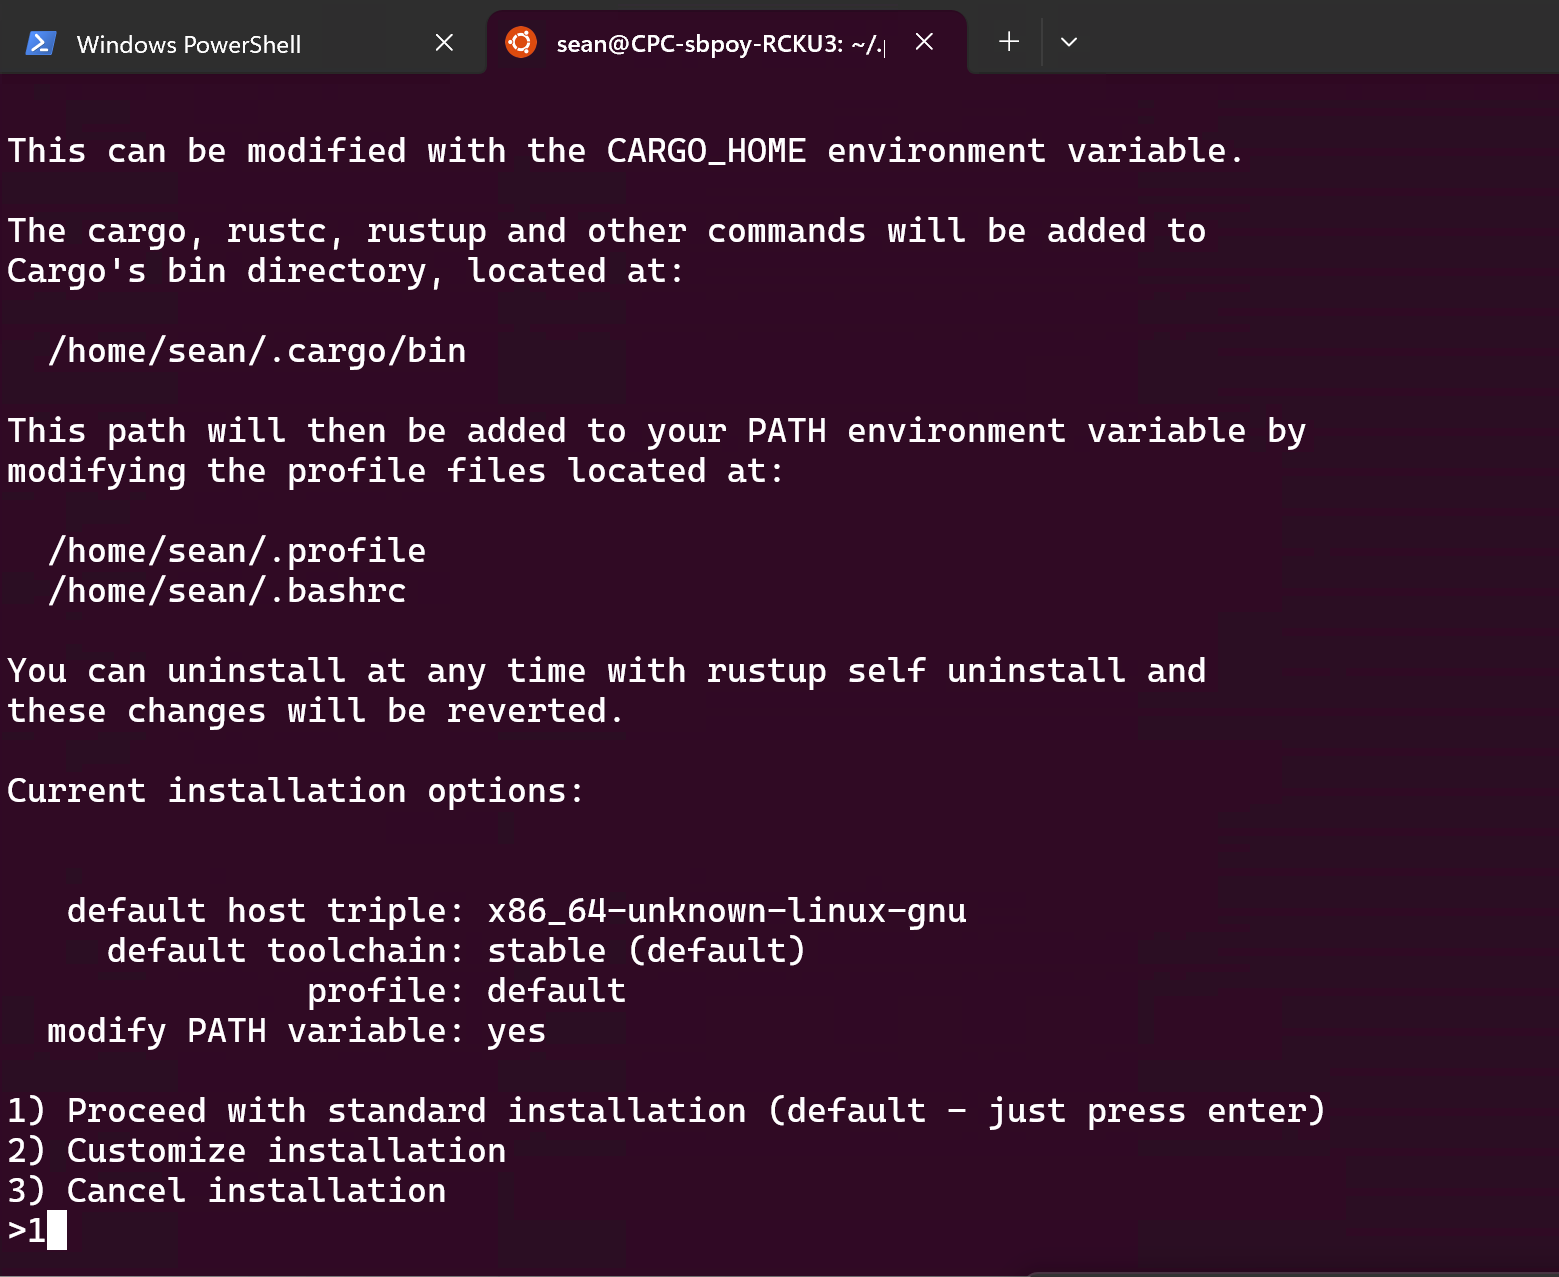
\includegraphics[width=0.85\textwidth]{slide03_img02.png}
\caption{Select option 1 to proceed with the default Rust installation.}
\end{figure}

After installation completes, activate the Rust environment and verify:

\begin{lstlisting}[style=bash]
source $HOME/.cargo/env
rustc --version
cargo --version
\end{lstlisting}

\begin{figure}[H]
\centering
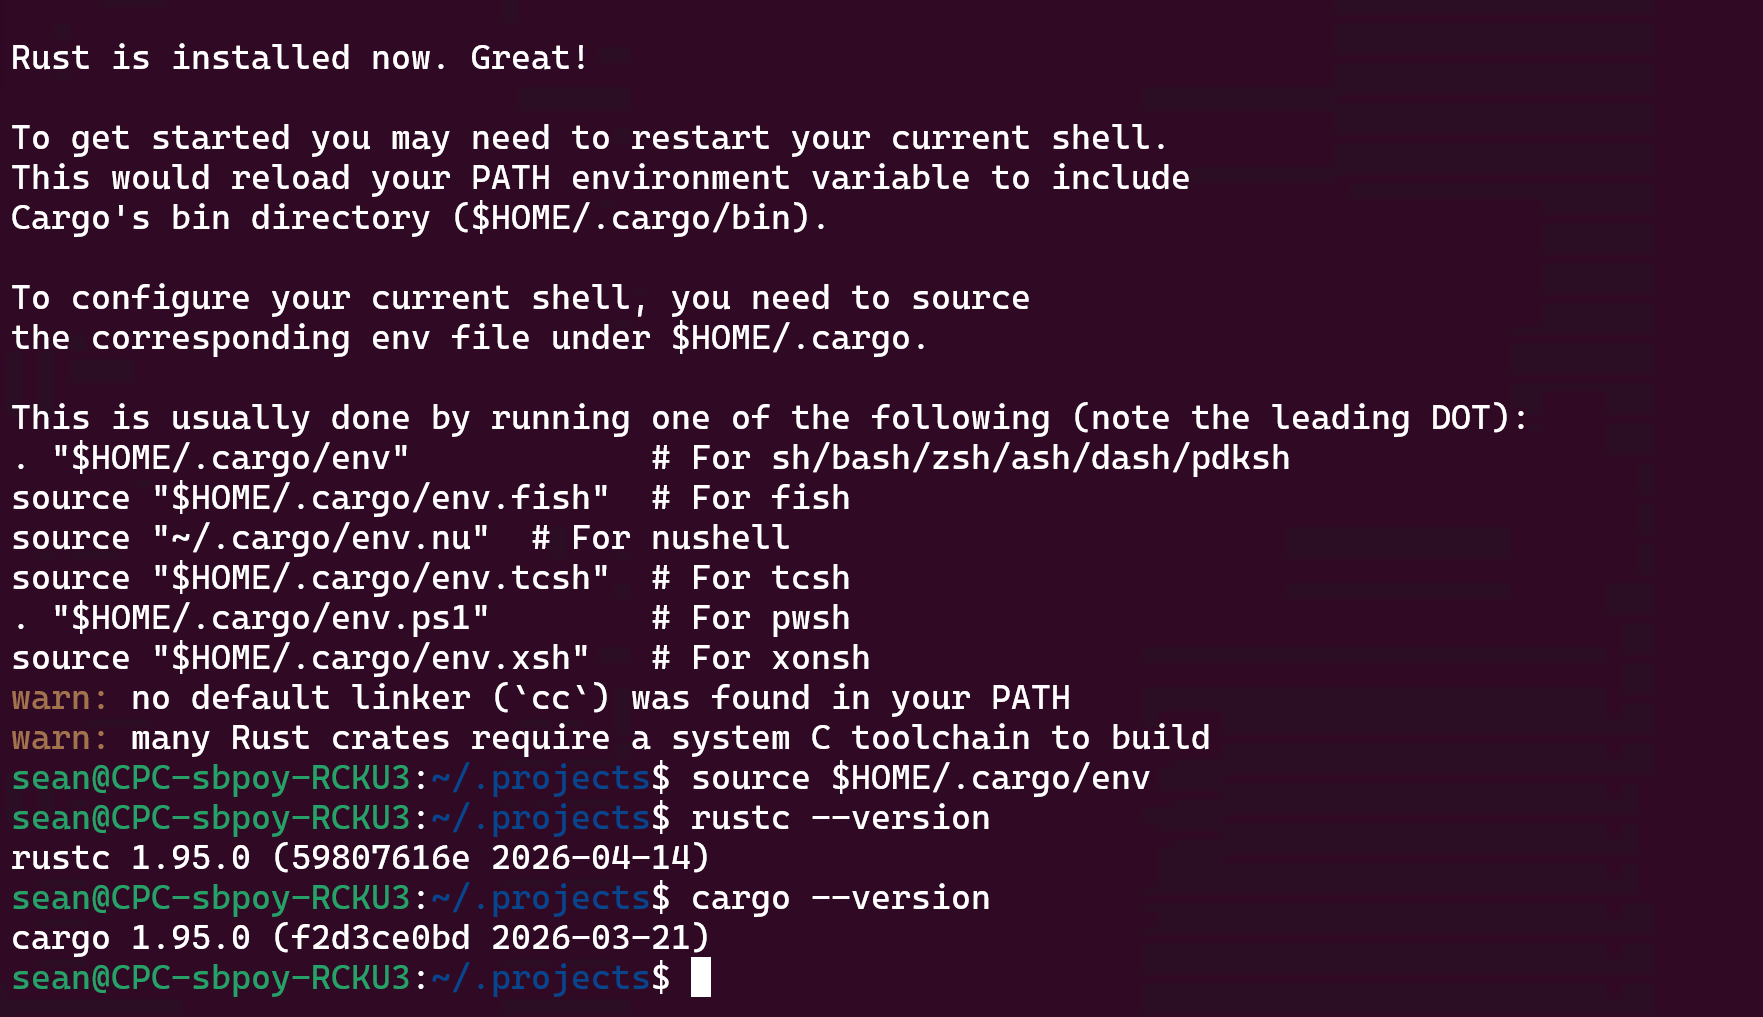
\includegraphics[width=0.85\textwidth]{slide04_img03.png}
\caption{Rust installed successfully. Note the \texttt{warn: no default linker
(`cc')} message --- this is expected if you haven't installed
\texttt{build-essential} yet (Step~2 resolves this).}
\end{figure}

\begin{tcolorbox}[tipbox={Tip}]
If you see \texttt{warn: no default linker (`cc') was found in your PATH},
make sure you completed Step~2 first. The Rust compiler needs a system C
linker to produce binaries.
\end{tcolorbox}

\newpage
% ============================================================================
\section{Step 4: Clone and Run the Installer}
% ============================================================================

Clone the LiteForge repository from GitHub Enterprise and run the installer
in a single command:

\begin{lstlisting}[style=bash]
git clone https://gitea.poyner.ai/sean/liteforge.git \
    /tmp/liteforge && \
    bash /tmp/liteforge/scripts/install.sh && \
    rm -rf /tmp/liteforge
\end{lstlisting}

You will be prompted for your GitHub Enterprise credentials:

\begin{figure}[H]
\centering
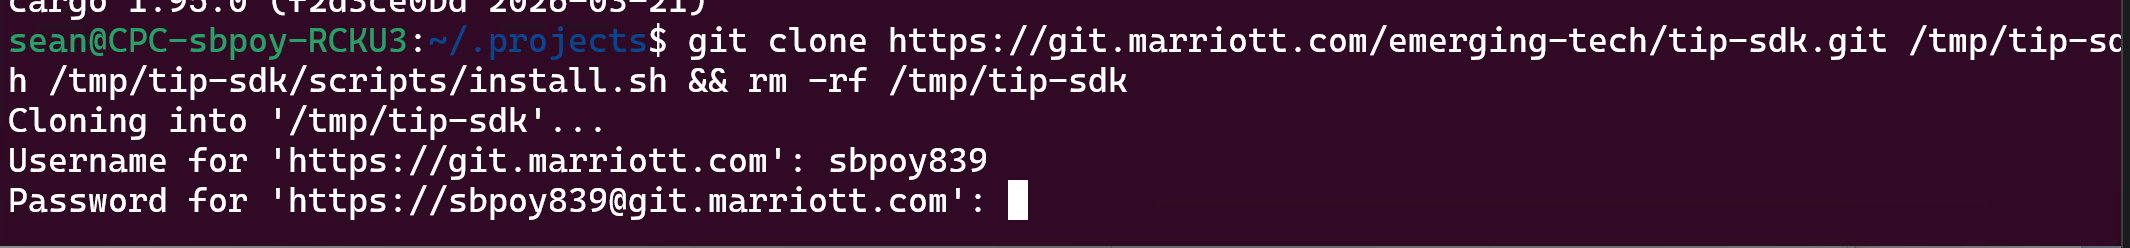
\includegraphics[width=0.85\textwidth]{slide05_img04.png}
\caption{Git clone prompts for GitHub Enterprise username and password.}
\end{figure}

The installer detects your platform, installs CA certificates, and begins
configuration:

\begin{figure}[H]
\centering
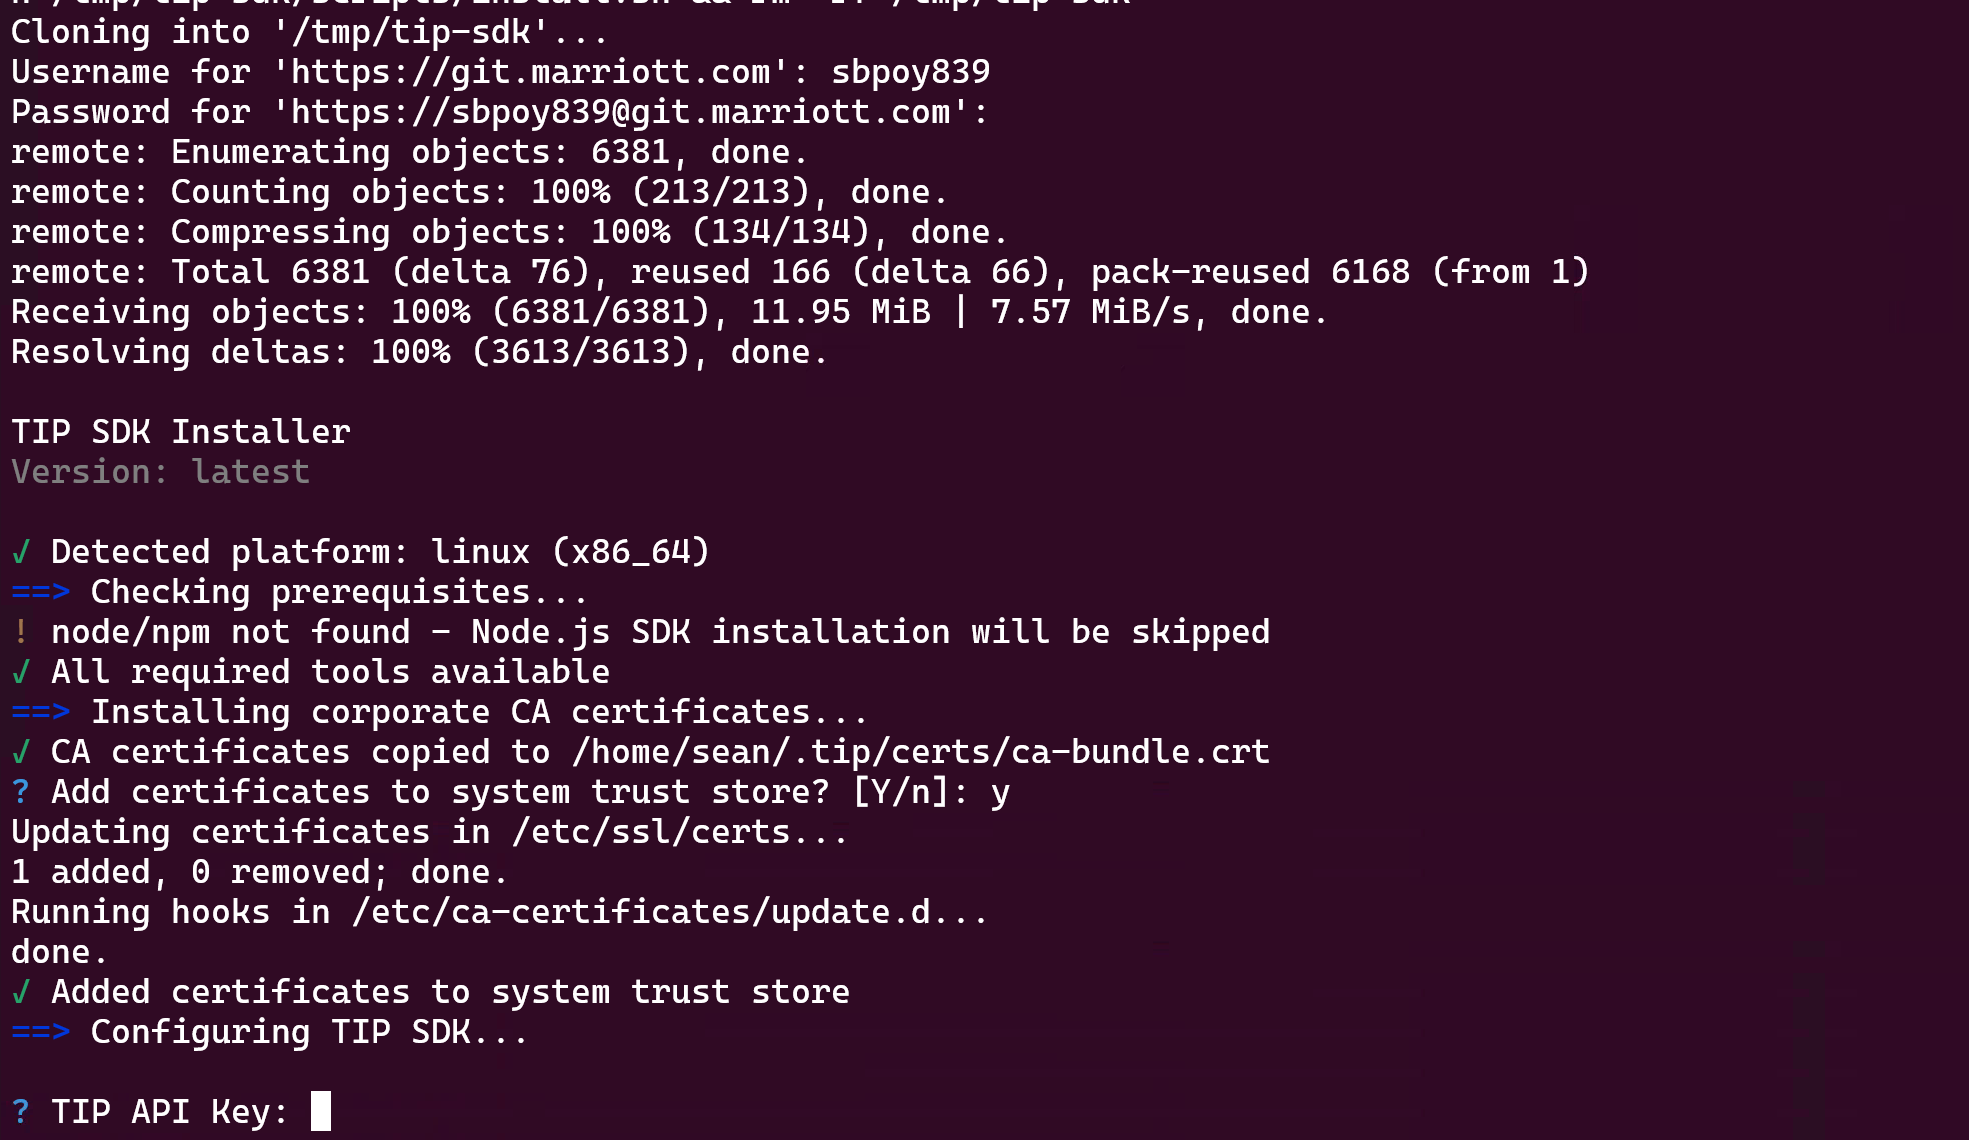
\includegraphics[width=0.85\textwidth]{slide06_img05.png}
\caption{The LiteForge Installer detects Linux x86\_64, installs corporate
CA certificates, and prompts for your API key.}
\end{figure}

\newpage
% ============================================================================
\section{Step 5: Configure LiteForge}
% ============================================================================

The installer prompts for your LiteForge configuration. Enter the values below
(press \textbf{Enter} to accept defaults shown in brackets):

\begin{table}[H]
\centering
\begin{tabularx}{0.9\textwidth}{@{}>{\bfseries}l X@{}}
\toprule
Prompt & What to enter \\
\midrule
LiteForge API Key & Your personal API key (required) \\
LiteForge Base URL & Press Enter for default \\
Default Model & Press Enter for \texttt{anthropic.claude-haiku-4-5-20251001-v1:0} \\
Knowledge Service URL & Press Enter to skip \\
Temporal Endpoint & Press Enter to skip \\
\bottomrule
\end{tabularx}
\caption{Installer configuration prompts and recommended values.}
\end{table}

\begin{figure}[H]
\centering
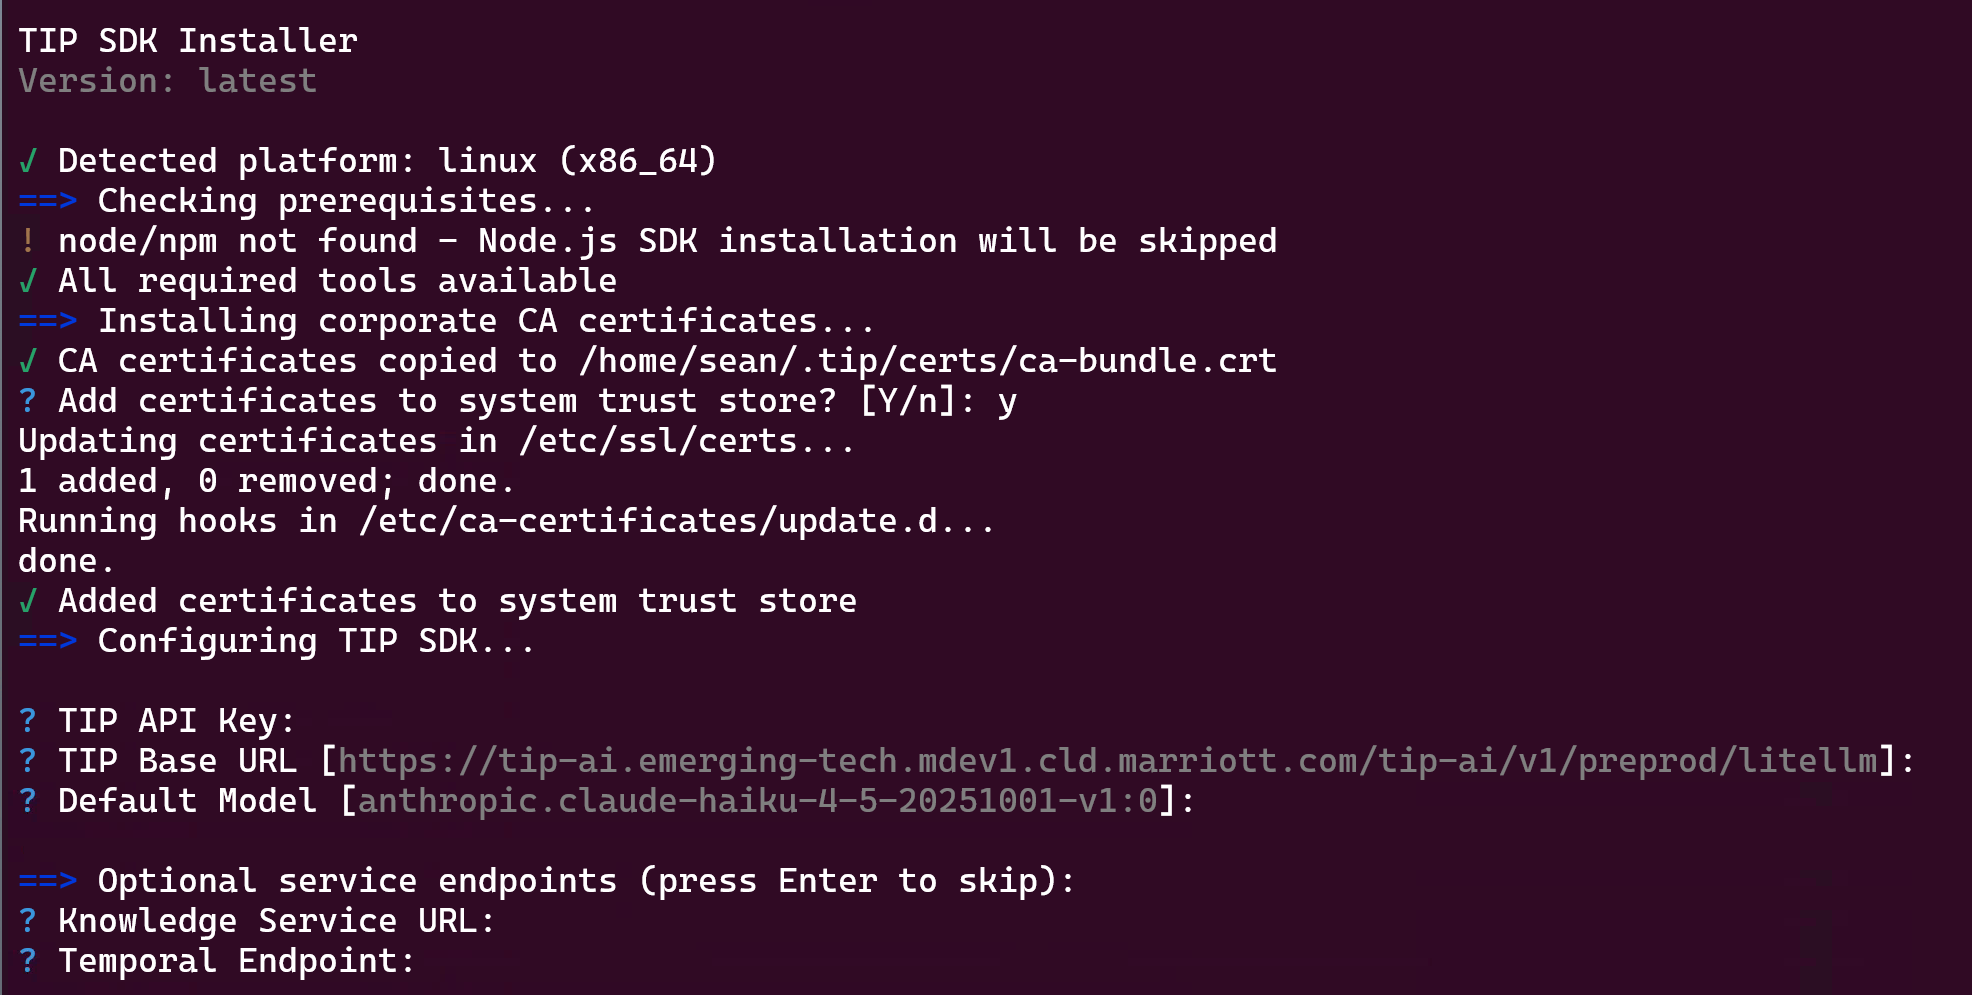
\includegraphics[width=0.85\textwidth]{slide07_img06.png}
\caption{Configuration prompts: API key, base URL, default model, and
optional service endpoints.}
\end{figure}

After credentials are validated, you select which components to install.
Answer \textbf{y} to the components you need:

\begin{figure}[H]
\centering
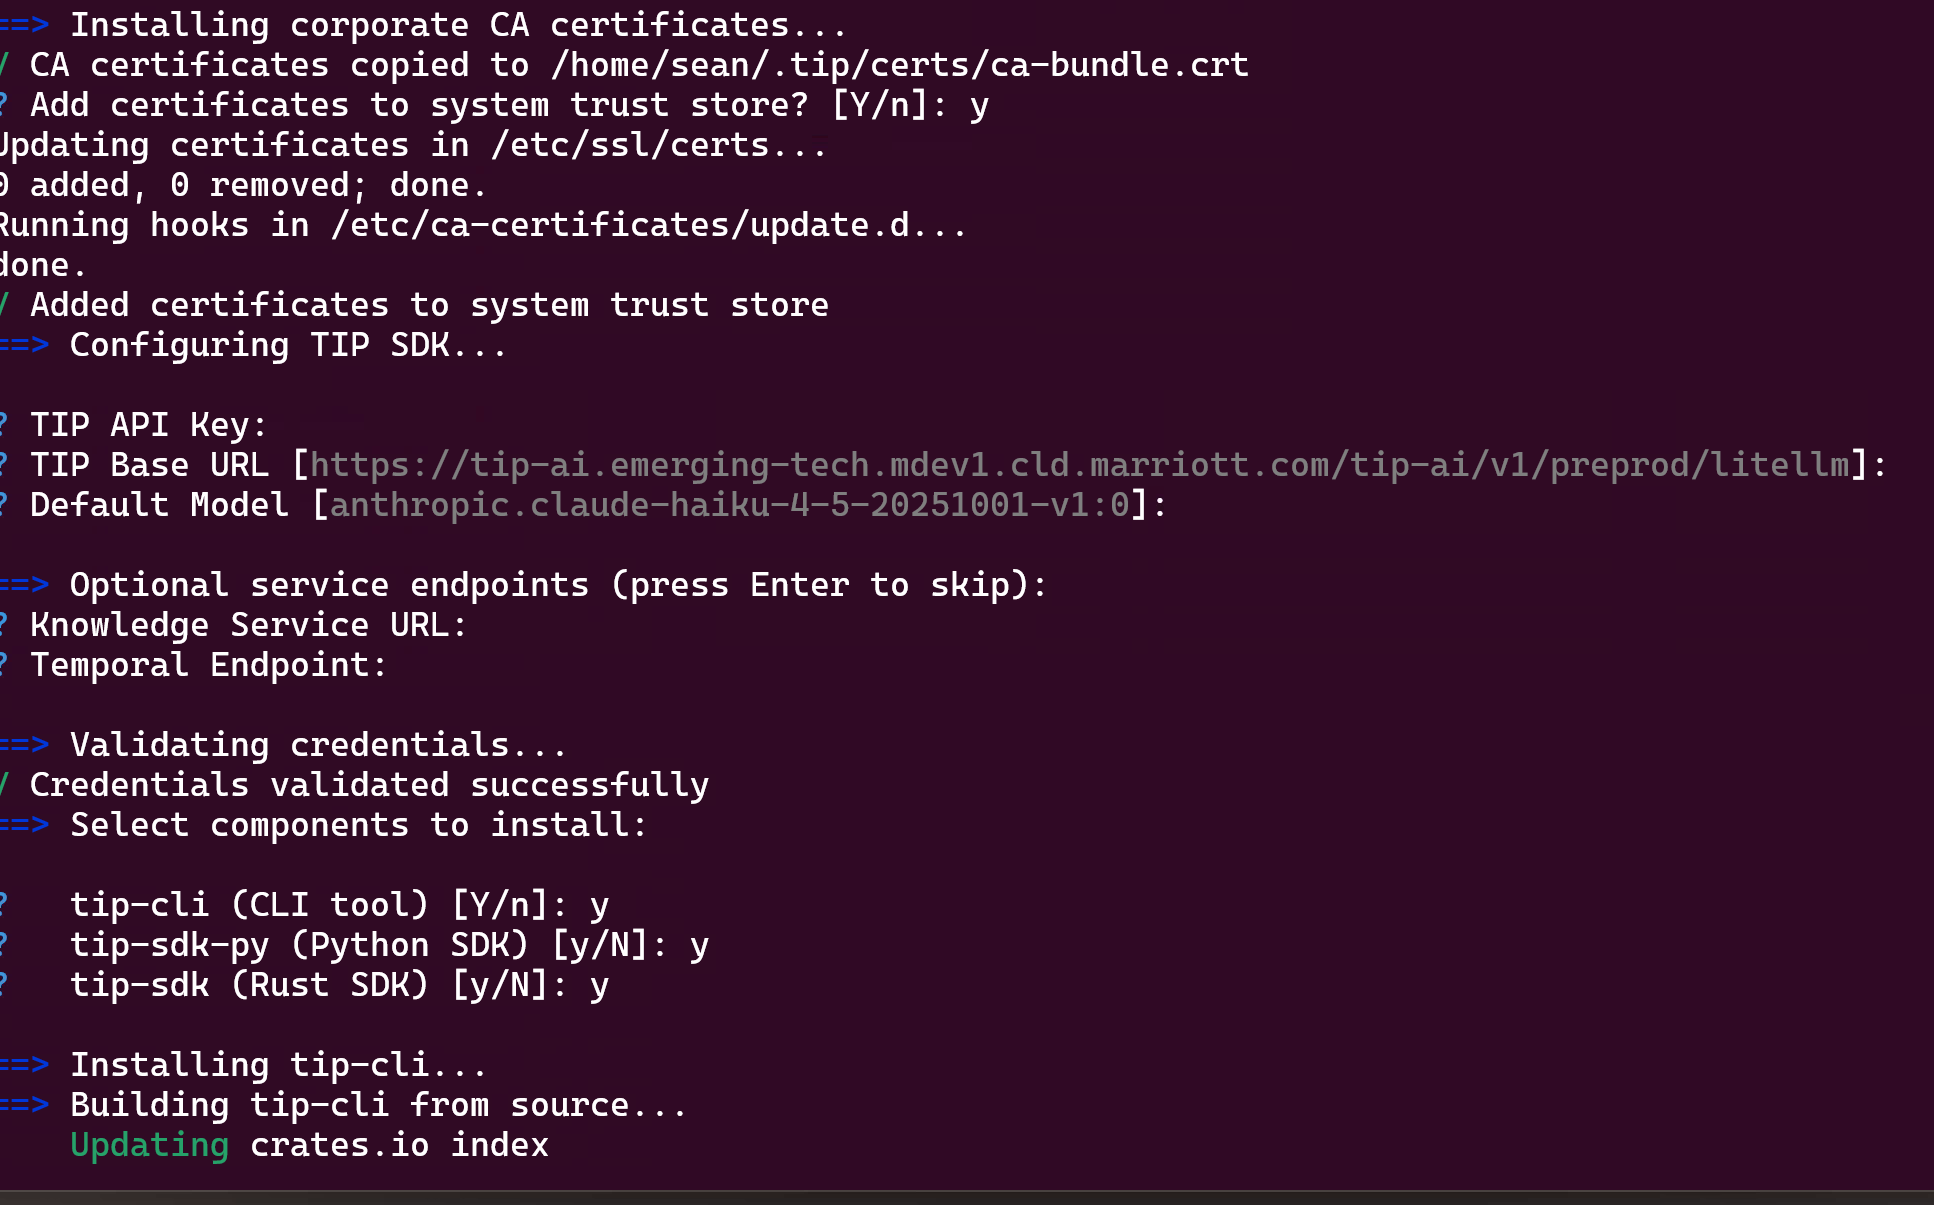
\includegraphics[width=0.85\textwidth]{slide08_img07.png}
\caption{Component selection: forge-cli (recommended), liteforge-py (Python SDK),
and liteforge (Rust SDK).}
\end{figure}

\subsection{Automatic Dependency Resolution}

The updated installer automatically handles missing system dependencies.
If the pre-built binary download is unavailable, it falls back to building
from source and detects missing tools:

\begin{figure}[H]
\centering
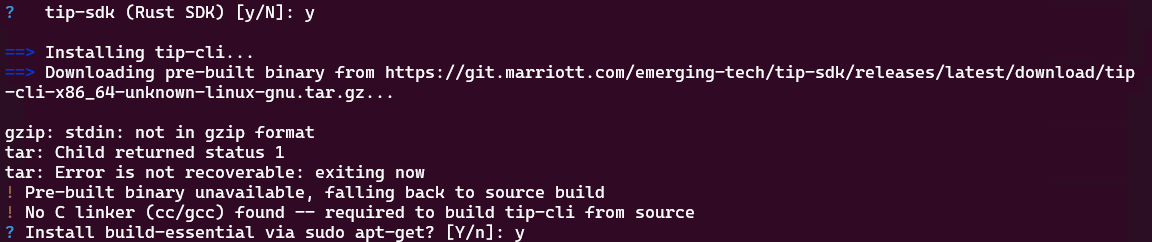
\includegraphics[width=0.85\textwidth]{slide09_img08.png}
\caption{The installer detects the missing C linker and offers to install
\texttt{build-essential} automatically. Answer \textbf{y}.}
\end{figure}

\begin{figure}[H]
\centering
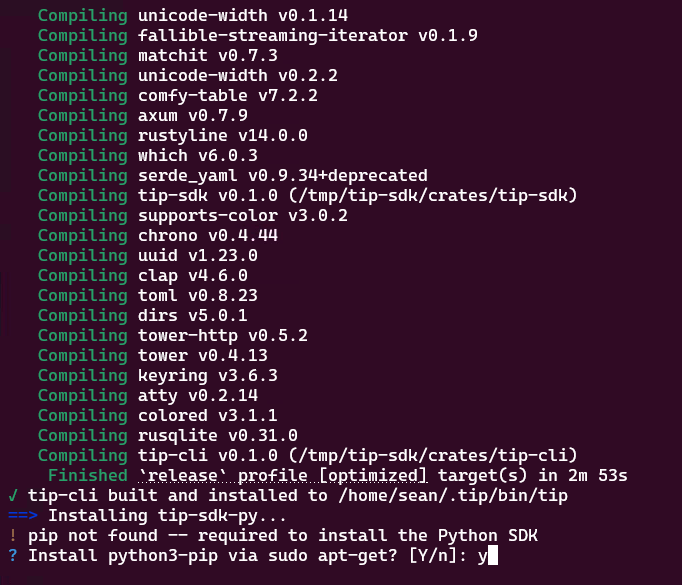
\includegraphics[width=0.85\textwidth]{slide10_img09.png}
\caption{The CLI builds successfully (2--3 minutes). The installer then
detects missing \texttt{pip} and offers to install \texttt{python3-pip}.
Answer \textbf{y}.}
\end{figure}

\begin{figure}[H]
\centering
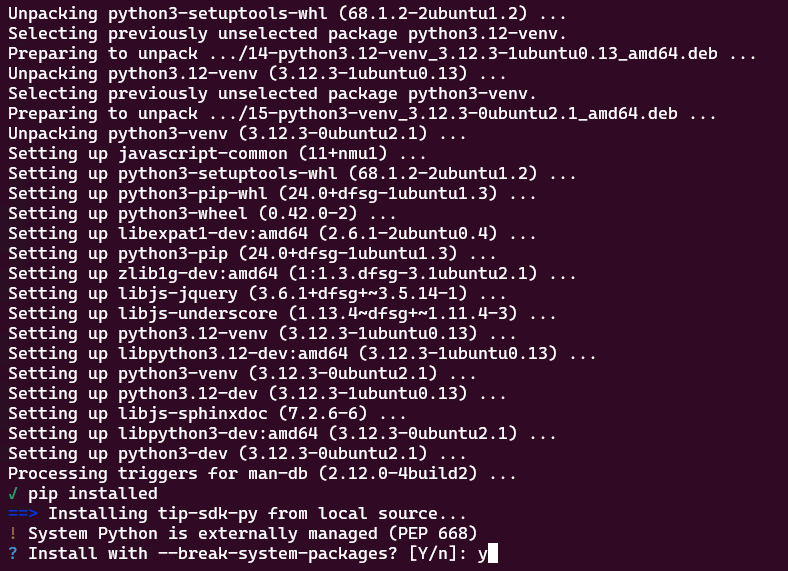
\includegraphics[width=0.85\textwidth]{slide11_img10.png}
\caption{\texttt{python3-pip} is installed and the Python SDK installation
proceeds. PEP~668 requires \texttt{--break-system-packages}; answer
\textbf{y}.}
\end{figure}

\begin{figure}[H]
\centering
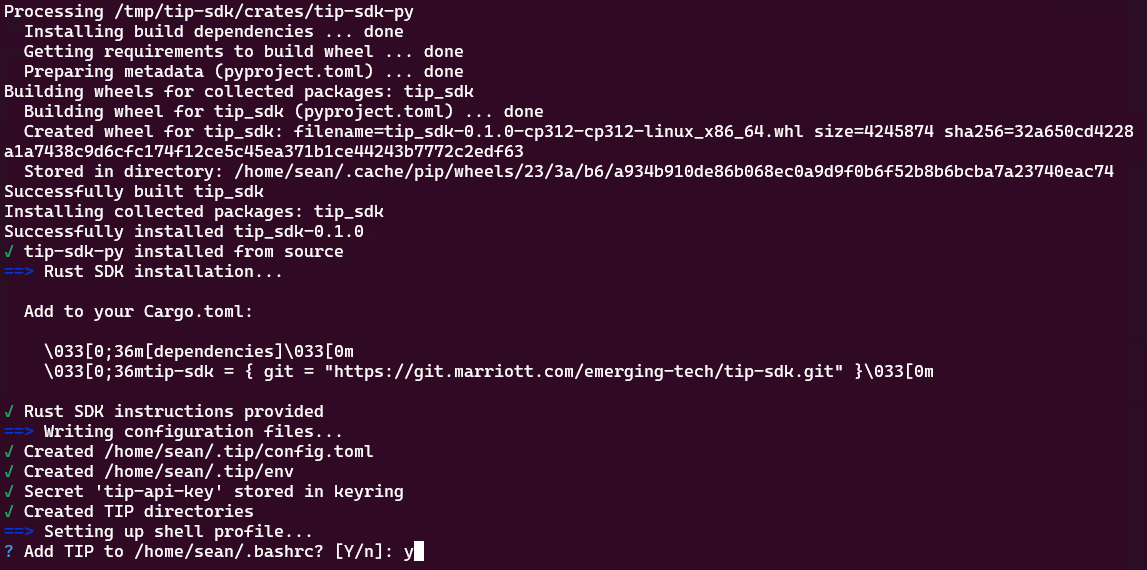
\includegraphics[width=0.85\textwidth]{slide12_img11.png}
\caption{Python SDK built and installed. Configuration files written.
Shell profile updated. Answer \textbf{y} to add LiteForge to
\texttt{\textasciitilde/.bashrc}.}
\end{figure}

\newpage
% ============================================================================
\section{Step 6: Verify Installation}
% ============================================================================

Source your updated shell profile and verify the \texttt{forge} CLI:

\begin{lstlisting}[style=bash]
source ~/.bashrc
forge --version
\end{lstlisting}

\begin{figure}[H]
\centering
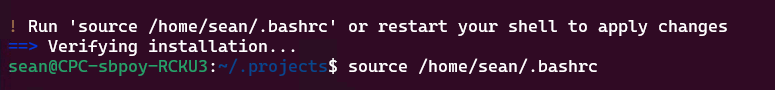
\includegraphics[width=0.6\textwidth]{slide13_img12.png}
\caption{Source the updated \texttt{.bashrc} to load LiteForge into your PATH.}
\end{figure}

\begin{figure}[H]
\centering
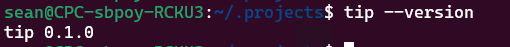
\includegraphics[width=0.45\textwidth]{slide13_img13.png}
\caption{\texttt{forge --version} reports \texttt{forge 0.1.0} ---
installation successful.}
\end{figure}

Run \texttt{forge --help} to see the full command list:

\begin{figure}[H]
\centering
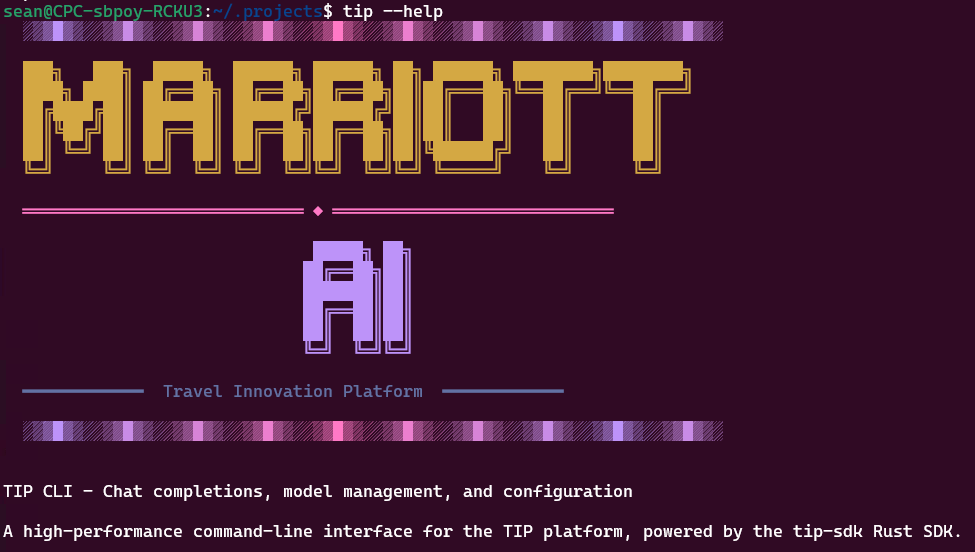
\includegraphics[width=0.85\textwidth]{slide14_img14.png}
\caption{The \texttt{forge --help} output with the Forge banner.}
\end{figure}

\begin{tcolorbox}[tipbox={Quick Test}]
Try your first chat completion:
\begin{lstlisting}[style=bash]
forge chat "What is the capital of France?"
\end{lstlisting}
If this returns a response, your API key and network connectivity are
working correctly.
\end{tcolorbox}

\newpage
% ============================================================================
\section{Step 7: Install and Launch Claude Code}
% ============================================================================

The \texttt{forge claude} command launches Claude Code with LiteForge environment
variables and a local proxy pre-configured. First, install Claude Code:

\begin{lstlisting}[style=bash]
curl -fsSL https://claude.ai/install.sh | bash
\end{lstlisting}

Add the install location to your PATH. Use the file that matches your
shell (\texttt{.bashrc} for bash, \texttt{.zshrc} for zsh on macOS):

\begin{lstlisting}[style=bash]
# Linux / WSL (bash)
echo 'export PATH="$HOME/.local/bin:$PATH"' >> ~/.bashrc
source ~/.bashrc

# macOS (zsh, default since macOS Catalina)
echo 'export PATH="$HOME/.local/bin:$PATH"' >> ~/.zshrc
source ~/.zshrc
\end{lstlisting}

\begin{figure}[H]
\centering
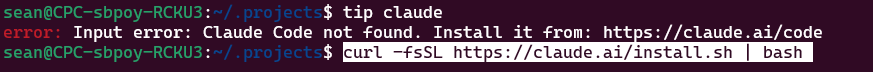
\includegraphics[width=0.85\textwidth]{slide15_img15.png}
\caption{If Claude Code is not installed, \texttt{forge claude} shows the
install command. Run the curl one-liner.}
\end{figure}

\begin{figure}[H]
\centering
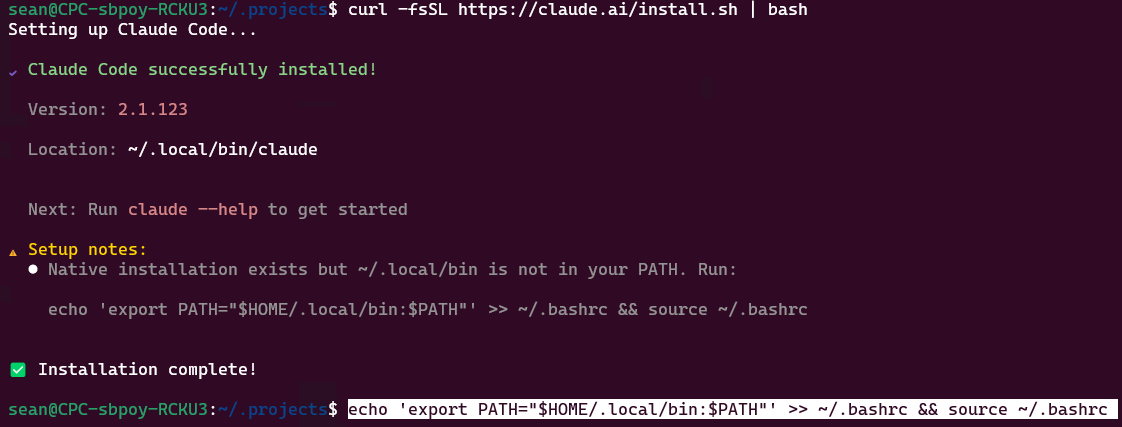
\includegraphics[width=0.85\textwidth]{slide15_img16.png}
\caption{Claude Code installs to \texttt{\textasciitilde/.local/bin/claude}.
Add it to your PATH.}
\end{figure}

Now launch Claude Code through LiteForge:

\begin{lstlisting}[style=bash]
forge claude
\end{lstlisting}

\begin{figure}[H]
\centering
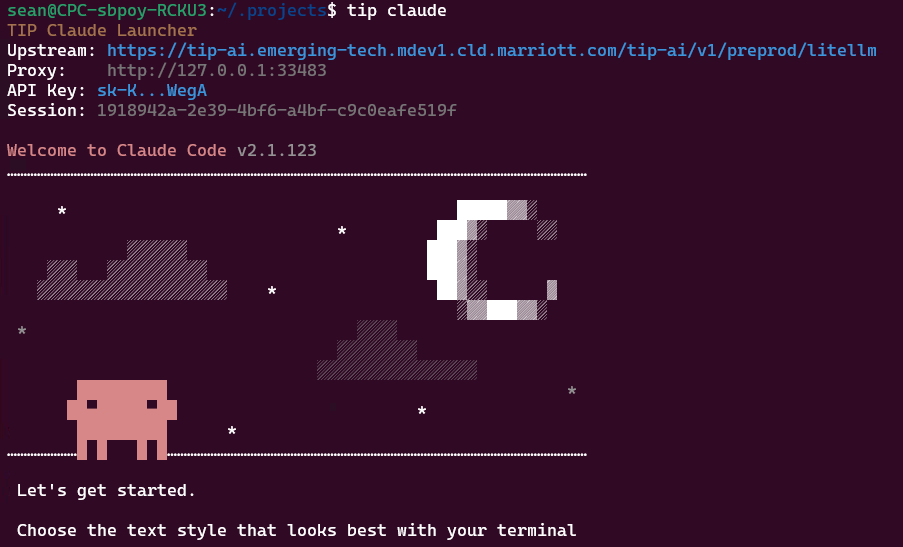
\includegraphics[width=0.85\textwidth]{slide16_img17.png}
\caption{\texttt{forge claude} starts a local proxy, injects the LiteForge API key
as \texttt{ANTHROPIC\_API\_KEY}, and launches Claude Code.}
\end{figure}

Claude Code will prompt you to accept the detected API key and trust the
workspace:

\begin{figure}[H]
\centering
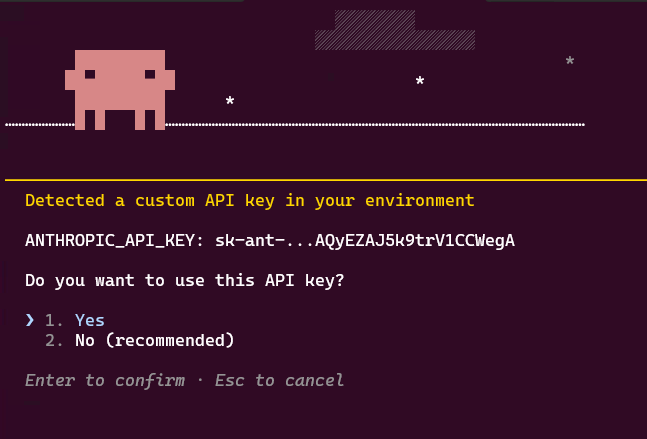
\includegraphics[width=0.75\textwidth]{slide17_img18.png}
\caption{Claude Code detects the LiteForge API key. Select \textbf{1. Yes} to
use it.}
\end{figure}

\begin{figure}[H]
\centering
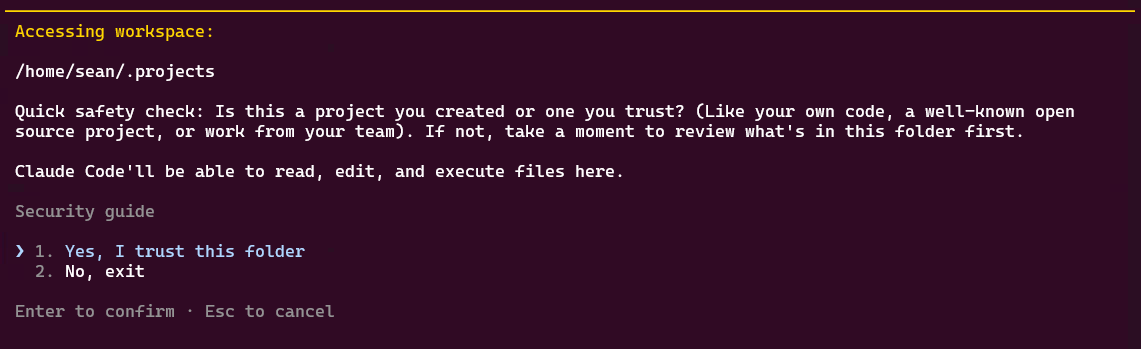
\includegraphics[width=0.85\textwidth]{slide17_img19.png}
\caption{Trust the workspace by selecting \textbf{1. Yes, I trust this
folder}.}
\end{figure}

\begin{figure}[H]
\centering
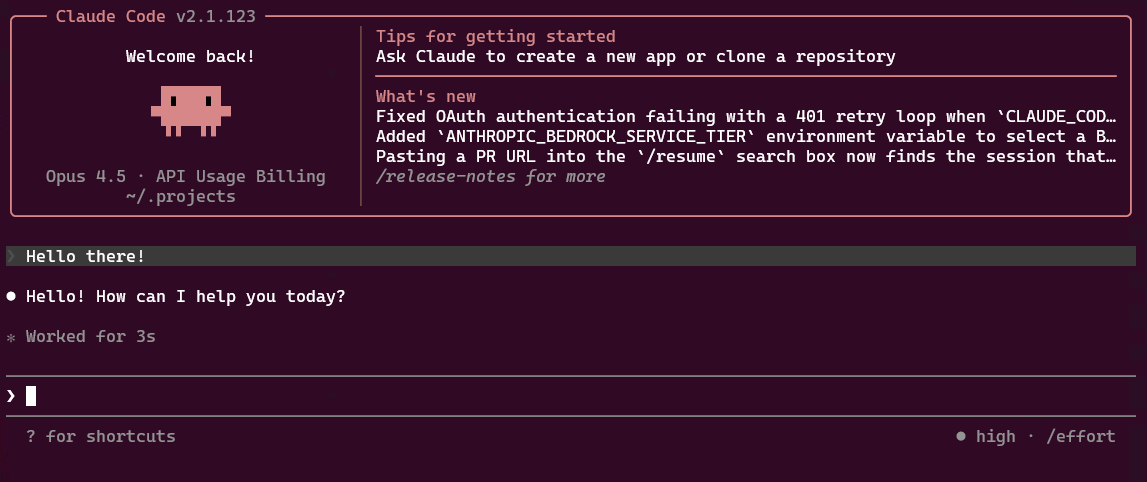
\includegraphics[width=0.85\textwidth]{slide18_img20.png}
\caption{Claude Code is running and ready. Try saying ``Hello there!''
to verify.}
\end{figure}

\begin{tcolorbox}[infobox={How it works}]
\texttt{forge claude} starts a local HTTP proxy that strips
\texttt{context\_management} fields and \texttt{context-management-*} beta
headers that LiteForge's LiteLLM rejects. This allows Claude Code to work
unmodified against the LiteForge gateway. Your API key flows through:
\texttt{\textasciitilde/.forge/config.toml} $\to$ \texttt{forge claude}
$\to$ \texttt{ANTHROPIC\_API\_KEY} env var $\to$ Claude Code.
\end{tcolorbox}

\newpage
% ============================================================================
\section{Step 8: Agent Development Kit (Bonus)}
% ============================================================================

The Forge CLI includes an Agent Development Kit (ADK) for scaffolding
containerized agent projects:

\begin{lstlisting}[style=bash]
forge adk --help
\end{lstlisting}

\begin{figure}[H]
\centering
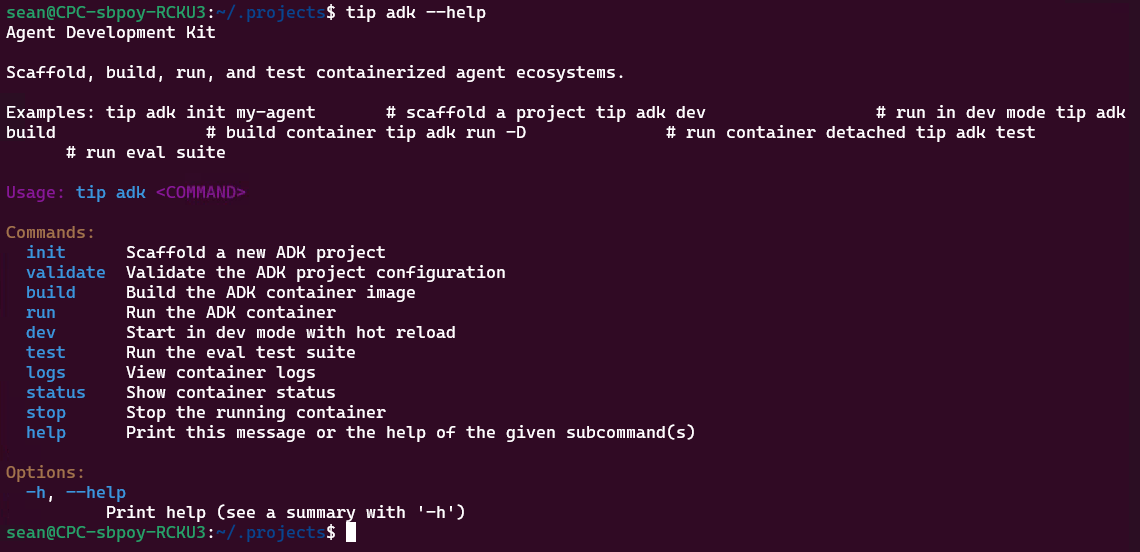
\includegraphics[width=0.85\textwidth]{slide19_img21.png}
\caption{\texttt{forge adk --help} shows available ADK commands.}
\end{figure}

Scaffold a new agent project:

\begin{lstlisting}[style=bash]
forge adk init my-agent
\end{lstlisting}

\begin{figure}[H]
\centering
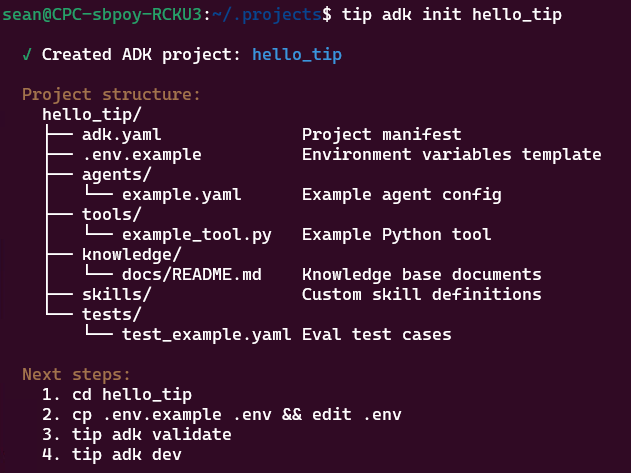
\includegraphics[width=0.75\textwidth]{slide20_img22.png}
\caption{\texttt{forge adk init} creates a complete project structure with
agent YAML configs, Python tools, knowledge base, and eval tests.}
\end{figure}

\newpage
% ============================================================================
\section{Troubleshooting}
% ============================================================================

\subsection{Claude Code keeps prompting for login (macOS)}

\begin{tcolorbox}[warnbox={Symptom}]
\texttt{forge claude} sets \texttt{ANTHROPIC\_API\_KEY} and
\texttt{ANTHROPIC\_BASE\_URL} correctly, but Claude Code ignores them and
keeps showing the login flow. Most common on macOS where Claude Code's
own config files (in \texttt{\textasciitilde/.claude.json} and
\texttt{\textasciitilde/.claude/settings.json}) override the environment
variables.
\end{tcolorbox}

\textbf{Cause:} Claude Code stores its API-key approval and base URL in
two JSON files. If your LiteForge key isn't in the \texttt{approved} list, or
if the global \texttt{anthropicBaseUrl} isn't set, Claude Code falls back
to the login flow even though the env vars are present.

\textbf{Fix:} Edit two files. Replace
\texttt{YOUR\_FULL\_TIP\_API\_KEY} with the real value (starts with
\texttt{sk-z-}) and \texttt{YOUR\_KEY\_SUFFIX\_HERE} with the last
$\sim$20 characters of that key.

\textbf{1. \texttt{\textasciitilde/.claude.json}} --- add your key
suffix to the approved list:

\begin{lstlisting}[style=bash]
{
  "customApiKeyResponses": {
    "approved": [
      "YOUR_KEY_SUFFIX_HERE"
    ],
    "rejected": []
  }
  // ... other existing fields preserved ...
}
\end{lstlisting}

\textbf{2. \texttt{\textasciitilde/.claude/settings.json}} --- add
\texttt{apiKeyHelper} and \texttt{anthropicBaseUrl}:

\begin{lstlisting}[style=bash]
{
  "theme": "dark",
  "apiKeyHelper": "echo 'YOUR_FULL_LITEFORGE_API_KEY'",
  "anthropicBaseUrl": "https://api.example.com/v1"
}
\end{lstlisting}

\begin{tcolorbox}[infobox={Why two files?}]
\begin{itemize}[nosep]
  \item \texttt{\textasciitilde/.claude.json} tracks which API keys
    Claude Code has been approved to send to. If your LiteForge key is in
    \texttt{rejected} (or missing), Claude Code refuses to use it and
    prompts for login.
  \item \texttt{\textasciitilde/.claude/settings.json} is the global
    settings file. \texttt{apiKeyHelper} is the command Claude Code runs
    to fetch the API key (env vars are overridden by this when set).
    \texttt{anthropicBaseUrl} points the SDK at the LiteForge gateway
    instead of \texttt{api.anthropic.com}.
\end{itemize}
After saving both files, \texttt{forge claude} starts immediately with no
login prompts.
\end{tcolorbox}

\subsection{``linker `cc' not found''}

\begin{tcolorbox}[warnbox={Error}]
\texttt{error: linker `cc' not found} \\
\texttt{note: No such file or directory (os error 2)}
\end{tcolorbox}

\textbf{Cause:} The system C toolchain is not installed. Rust requires
\texttt{cc}/\texttt{gcc}/\texttt{clang} to link native code.

\textbf{Fix (Linux / WSL):}
\begin{lstlisting}[style=bash]
sudo apt-get install -y build-essential pkg-config libssl-dev
\end{lstlisting}

\textbf{Fix (macOS):}
\begin{lstlisting}[style=bash]
xcode-select --install
brew install pkg-config openssl@3
\end{lstlisting}

\subsection{``No module named pip''}

\begin{tcolorbox}[warnbox={Error}]
\texttt{/usr/bin/python3: No module named pip} \\
\texttt{Failed to install Python SDK from source}
\end{tcolorbox}

\textbf{Cause:} Modern Ubuntu ships \texttt{python3} without \texttt{pip}.
On macOS this happens when only the system Python is installed (no pip
shipped).

\textbf{Fix (Linux / WSL):}
\begin{lstlisting}[style=bash]
sudo apt-get install -y python3-pip python3-venv
\end{lstlisting}

\textbf{Fix (macOS):}
\begin{lstlisting}[style=bash]
brew install python@3.12
\end{lstlisting}

\subsection{``Certificate verify failed''}

\textbf{Cause:} Corporate proxy or missing CA certificates.

\textbf{Fix:} The installer should have installed the CA bundle
automatically. Verify:
\begin{lstlisting}[style=bash]
ls ~/.forge/certs/ca-bundle.crt
echo $SSL_CERT_FILE
\end{lstlisting}

If the cert file is missing, re-run the installer or manually copy the
certificate bundle from the repository:
\begin{lstlisting}[style=bash]
mkdir -p ~/.forge/certs
cp /tmp/liteforge/certs/combined-full-ca-bundle.crt \
   ~/.forge/certs/ca-bundle.crt
\end{lstlisting}

\subsection{Proxy / Netskope Issues}

If you encounter TLS errors when Rust downloads crates from
\texttt{crates.io}, set the cargo revocation check override:

\begin{lstlisting}[style=bash]
export CARGO_HTTP_CHECK_REVOKE=false
\end{lstlisting}

Add this to \texttt{\textasciitilde/.bashrc} to make it permanent.

\newpage
% ============================================================================
\section{Quick Reference}
% ============================================================================

\begin{table}[H]
\centering
\renewcommand{\arraystretch}{1.3}
\begin{tabularx}{\textwidth}{@{}>{\ttfamily\small}l X@{}}
\toprule
\textnormal{\textbf{Command}} & \textbf{Description} \\
\midrule
forge chat "..." & Chat with an LLM \\
forge chat -i & Interactive REPL mode \\
forge chat --stream "..." & Streaming response \\
forge models & List available models \\
forge config show & Display all settings \\
forge config set api-key KEY & Set API key \\
forge claude & Launch Claude Code with LiteForge config \\
forge agents & List available agents \\
forge tools & List agent tools \\
forge embed "text" & Generate embeddings \\
forge chunk "text" & Split text into chunks \\
forge guardrails "text" & Check for PII / prompt injection \\
forge serve & Start multi-port agent server \\
forge adk init NAME & Scaffold an agent project \\
forge adk dev & Hot-reload dev server \\
forge adk build & Build container image \\
forge usage & View API usage reports \\
\bottomrule
\end{tabularx}
\caption{Forge CLI command quick reference.}
\end{table}

\begin{tcolorbox}[infobox={Configuration Locations}]
\begin{tabularx}{\textwidth}{@{}>{\ttfamily\small}l X@{}}
\textasciitilde/.forge/config.toml & Main configuration (API key, base URL, model) \\
\textasciitilde/.forge/env & Shell environment variables (sourced by .bashrc) \\
\textasciitilde/.forge/certs/ca-bundle.crt & Corporate CA certificate bundle \\
\textasciitilde/.forge/bin/forge & CLI binary location \\
\end{tabularx}
\end{tcolorbox}

\vfill

\begin{center}
\small\color{forgegray}
\rule{0.6\textwidth}{0.4pt}\\[6pt]
LiteForge v0.1.0 -- LiteForge\\
\textcolor{alertred}{\textit{Proprietary and Confidential}}
\end{center}

\end{document}
